%\vspace{-2mm}
\section{Methods for Legal Retrieval} \label{sec:method}
%\vspace{-3mm}
As a baseline, we experimented with an array of methods: lexical and semantic in supervised and unsupervised settings and summary based methods.  
%We try out a variety of methods, both supervised and unsupervised, for the two retrieval tasks.  Some of these methods focus on lexical matching via n-grams, while other methods focus on the semantic features, using dense representations from deep neural models. Also, we try out summary-based and paragraph-level methods, as described below. 
%that utilize summaries / individual paragraphs instead of the long case judgments as queries/precedents.

%\subsection{Lexical Methods} \label{sec:method/lexical}
%\vspace{2mm}

\vspace{1mm}
\noindent\underline{\textbf{Lexical Methods:}} We experimented with methods based on BM25, a strong baseline for legal retrieval~\cite{joshi2023ucreat}). 
%\noindent\underline{\textbf{Lexical Methods:}} We experimented with lexical methods based on BM25 (a strong baseline for legal retrieval~\cite{joshi2023ucreat}). 

\noindent\textbf{1) BM25:} It is an unsupervised method relying on n-gram lexical matches between the query and candidates to generate scores~\citep{robertson2009bm25}. 
%It is an advanced version of the TF-IDF algorithm (unsupervised), relying on n-gram based lexical matches between the query and candidates to generate scores~\citep{robertson2009bm25}.

\begin{figure}[t]
    \centering
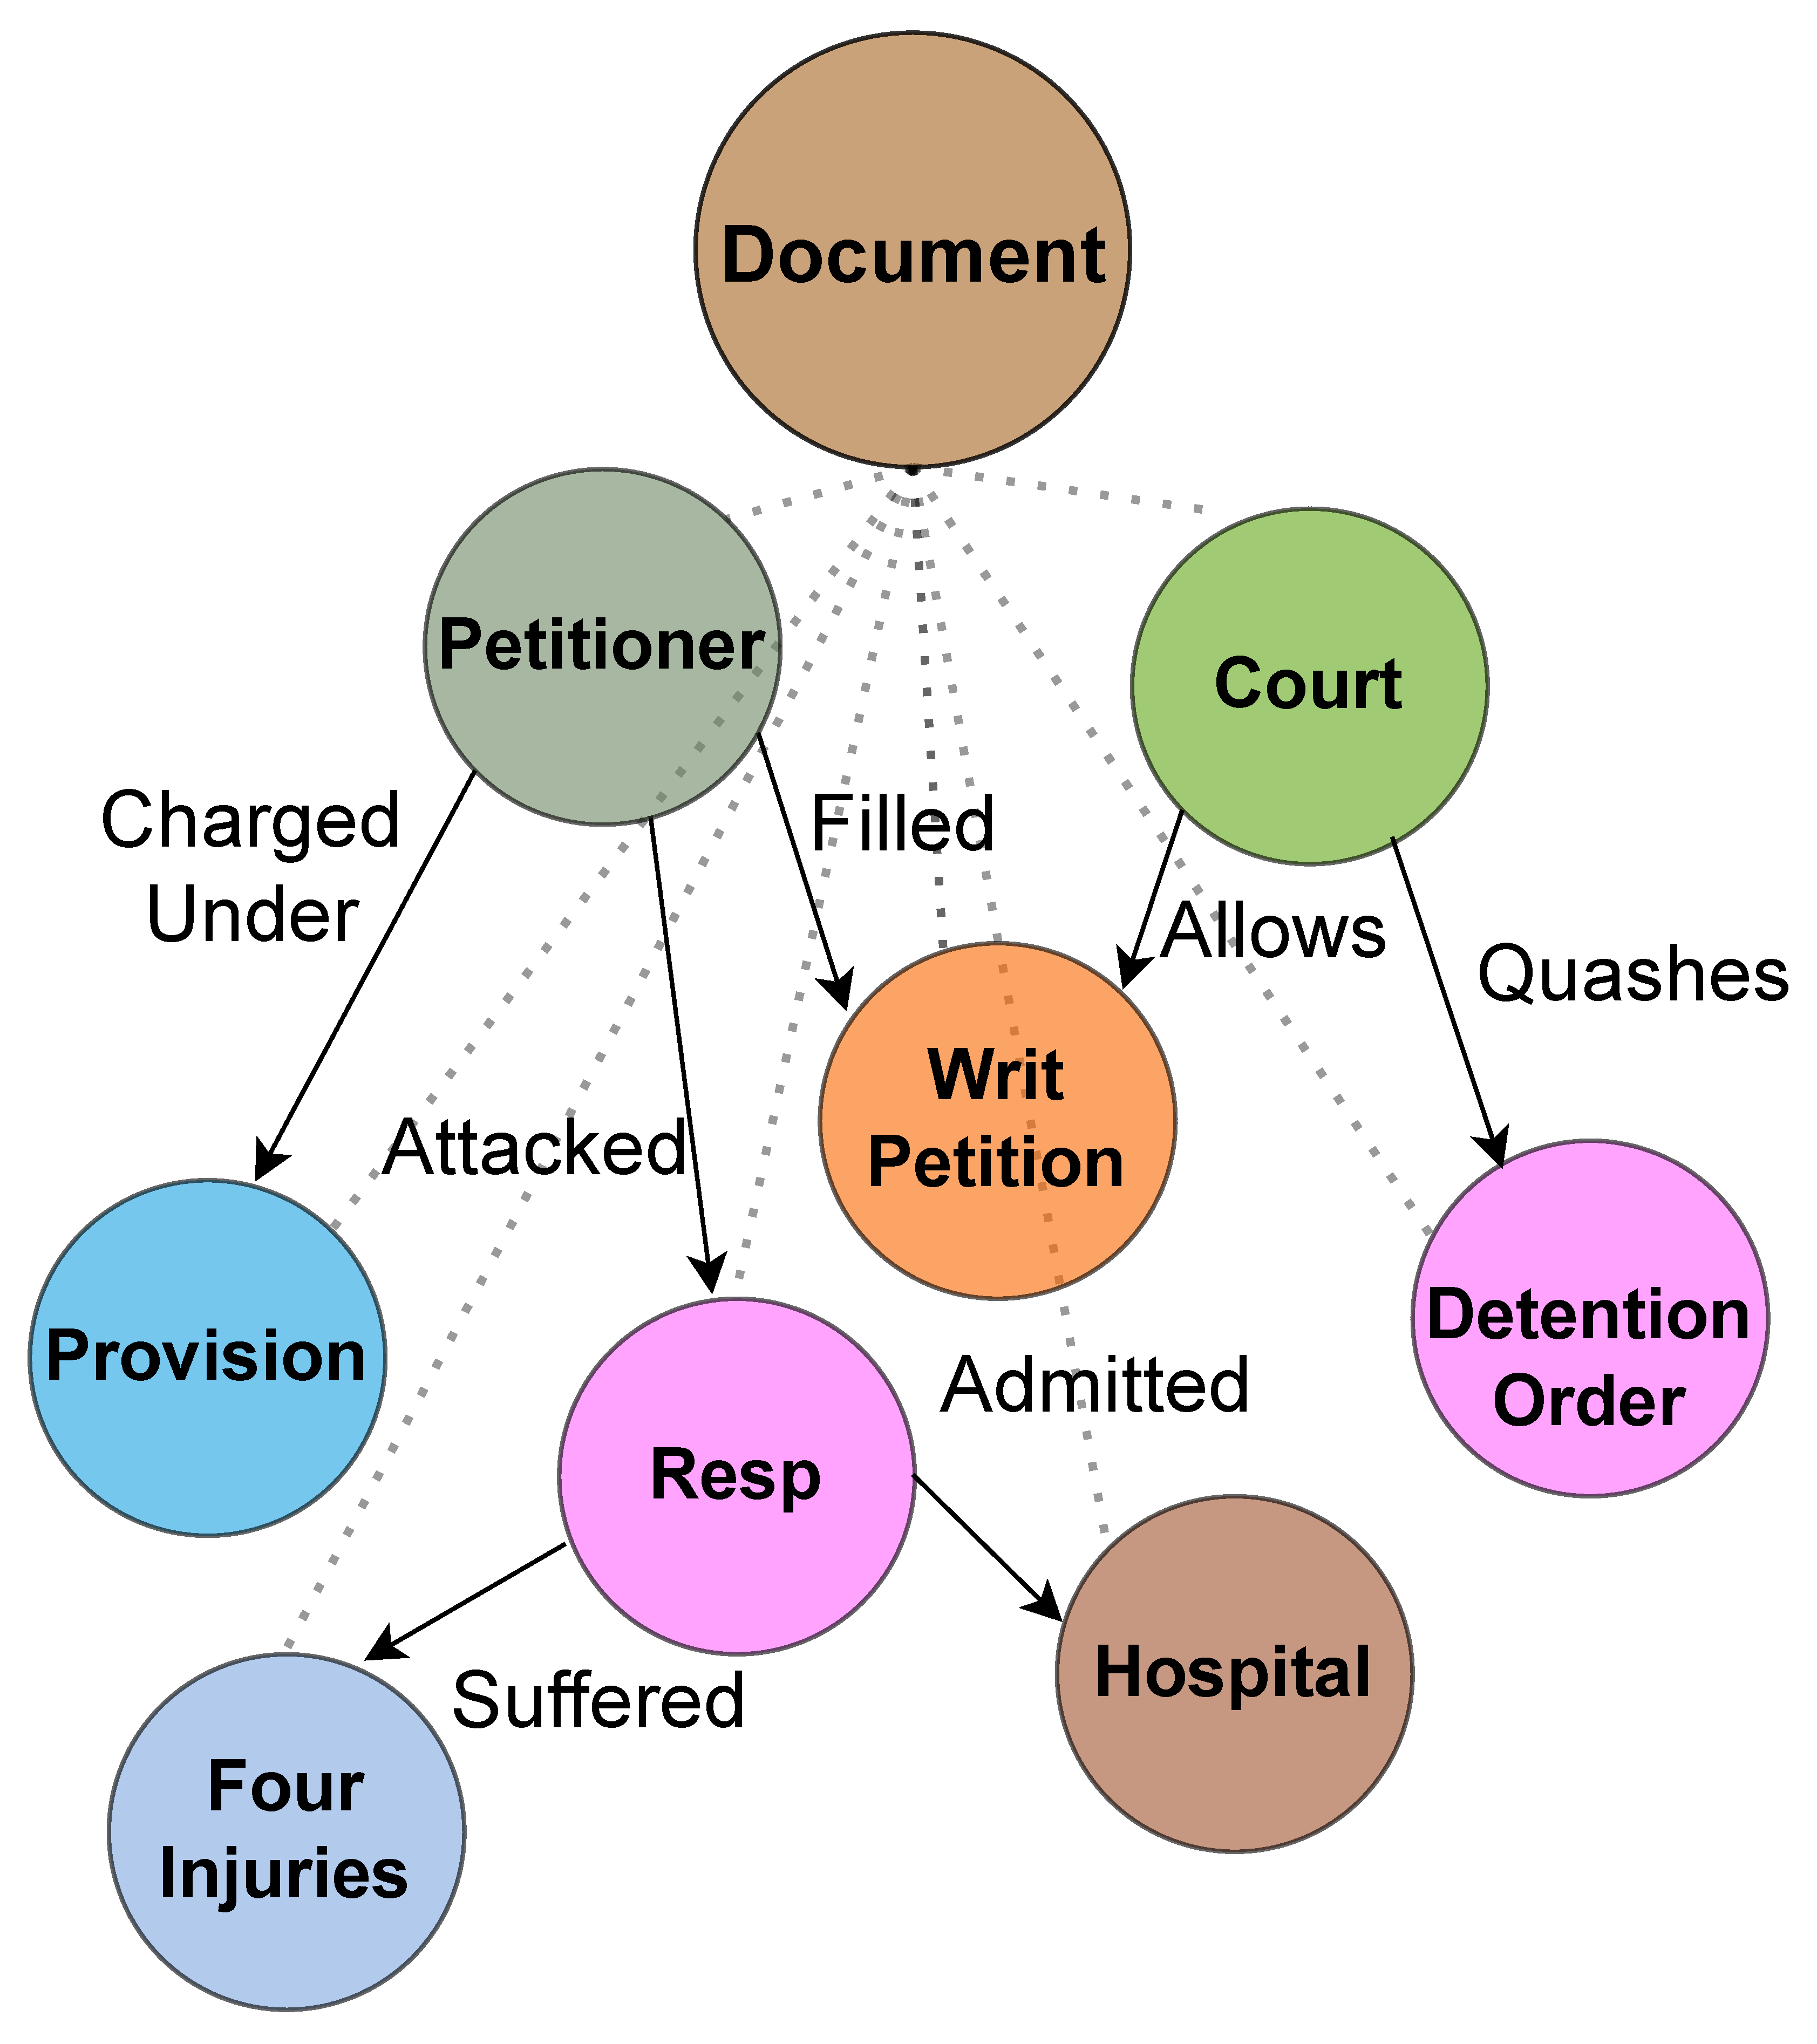
\includegraphics[scale=0.12,height=7cm]{./images/EventGNN.pdf}
    \vspace{-2mm}
    \caption{Part of the graph of a case document based on LLM-generated events (input for Event-GNN)}
    \label{fig:eventgnn}
    \vspace{-6mm}
\end{figure}

\noindent \textbf{2) SpaCy Events + BM25:} Prior works have demonstrated that both the queries and precedent candidates tend to be long and noisy, with only small portions of text leading to a strong match. \citet{joshi2023ucreat} used SpaCy (\url{www.spacy.io}) to extract events (subject, action, object triplets) and filtered out only the sentences containing matching events from both queries and precedents, leading to a better match. % via BM25. %We performed the same experiment.

\noindent\textbf{3) LLM Events + BM25:} We observed that SpaCy tends to over-generate events and is noisy. To address this, we employed an LLM (\texttt{gemma-7b-it}: \url{https://huggingface.co/google/gemma-7b-it}) to extract important events (prompt in Table~\ref{tab:event-llm-prompt}, App.~\ref{app:prompts}). We passed definitions from the SALI ontology (Standards Advancement for the Legal Industry: \url{https://www.sali.org/}) to guide the LLM in event generation. 
% We observed that LLM events are fewer than SpaCy events, but the elements in the (subject, action, object) triplets are larger (entire phrases/clauses) than that of SpaCy (one/two words at maximum). These events were subsequently used to filter out sentences for BM-25 baseline.
We found LLM events were fewer than SpaCy events but had larger triplet elements (subjects, actions, objects as full phrases/clauses vs. one–two words). These events were then used to filter sentences for the BM25 baseline.
%We observed that SpaCy generated a lot of events from a single query/candidate, which may not be ideal for the retrieval tasks. To customize this behavior, we employed an LLM (\texttt{gemma-7b-it}) to extract important events. We passed definitions from the SALI (Standards Advancement for the Legal Industry) (\url{https://www.sali.org/}) ontology to guide the LLM in event generation. We observed that LLM events are fewer than SpaCy events, but the elements in the (subject, action, object) triplets are larger (entire phrases/clauses) than that of SpaCy (one/two words at maximum). These events were subsequently used to filter out sentences for BM-25 baseline. % After extracting these events, we filtered out the sentences containing them and applied BM25 for the retrieval.

%\subsection{Semantic Methods} \label{sec:method/semantic}
%\vspace{2mm}
\vspace{1mm}
\noindent\underline{\textbf{Semantic Methods:}}
Semantic methods use deep-learning models trained on the train set. For fine-tuning, we explored two settings: (i)~training separate models for each task, and (ii)~a multi-task setup performing LSR and PCR simultaneously.

\noindent \textbf{1) SAILER:} \citet{li2023sailer} pre-trained a BERT-based model on legal documents to generate case reasoning and judgment from facts, then fine-tuned it for case retrieval on COLIEE 2021~\citep{rabelo2022coliee21}. We used this model for inference, with and without additional fine-tuning on our train set.


\noindent \textbf{2) Event-GNN:}
% Inspired by \citet{li2023findkg} we used GPT-4 (\texttt{gpt-4-turbo}: \url{https://platform.openai.com/docs/models/gpt-4-turbo})
% for creating event triplets for a small number ($\sim 400$) of documents from the train set and these triplets were subsequently used to fine-tune Gemma (\texttt{gemma-7b-it}) for generating triplets for the entire corpus. The triplets are used to create a graph with each subject and object being the nodes, and edges labeled with the action connecting the nodes (see App. Fig. \ref{fig:eventgnn}). 
% To reduce sparsity, we also introduced a global node to represent the whole document and connected each such global node with the global node of the cited case. All texts (corresponding to nodes (entity) and edges (relationships)) are encoded using SentenceBERT~\citep{reimers2019sentencebert}. We then employed a 2-layer Graph Attention Network~\citep{tang2024casegnn++} and perform dot product over the global nodes to capture document-level similarity between a query and candidate.
Inspired by \citet{li2023findkg}, we used GPT-4 (\texttt{gpt-4-turbo}: \url{https://platform.openai.com/docs/models/gpt-4-turbo}) to create event triplets for $\sim$400 training documents, then fine-tuned Gemma (\texttt{gemma-7b-it}) to generate triplets for the full corpus. Each triplet forms a graph where subjects/objects are nodes and actions label the edges (see Fig.~\ref{fig:eventgnn}). To reduce sparsity, a global node (connected to every subject/object node) represents each document and is linked to the global node of the cases it cites. Node (entity) and edge (relation) texts are encoded with SentenceBERT~\citep{reimers2019sentencebert}, and a 2-layer Graph Attention Network~\citep{tang2024casegnn++} computes document-level similarity via dot product over global nodes.


\noindent \textbf{3) Para-GNN:} 
% Different paragraphs in court case documents can usually be categorized into functional parts / rhetorical roles (from a legal perspective), such as Facts of the case, Arguments by lawyers, Ruling by the judge, etc.~\citep{malik-rr-2021}. The corpus source website IndianKanoon provides the rhetorical role for each paragraph, which can be used directly. Thus, we construct a setup where for each query/candidate, we have a global node representing the entire document and nodes for each paragraphs, connected to the global node with the edge labeled with the rhetorical role. The texts are converted to embeddings using SentenceBERT, and then a two-layer Graph Attention Network is employed on top. Dot product is calculated over the global nodes only. For statutes, each different subsection is taken as individual paragraphs, and the rhetorical role of each such paragraph is set to `None'.
Court case documents can be divided into segments such as Facts, Arguments, and Rulings~\citep{malik-rr-2021}, each performing a different rhetorical role from a legal perspective. IndianKanoon provides these labels per paragraph, which we use directly. For each query/candidate, we build a graph with a representative global node (whole document) and paragraph nodes linked to it via their rhetorical role. Texts are embedded with SentenceBERT, and a two-layer Graph Attention Network is applied, with dot product computed over global nodes. For statutes, each subsection is treated as a paragraph with role set to `None'.



%\subsection{Summary-based methods} \label{sec:method/summary}

\vspace{1mm}
%\vspace{2mm}
\noindent\underline{\textbf{Summary-based methods:}} 
% Using full case documents as both queries and precedents not only leads to large computation overload, but also introduces additional challenges for semantic models~\citep{tang2024caselink,tang2024casegnn++,qin2024ljpretrieval,yue2024eventcourtview}. 
% Full cases contain a lot of details that act as noise for statute and precedent retrieval. 
% Additionally, different portions of input text provide the contextual information needed for statute retrieval as compared to precedent retrieval. 
% Thus, we conducted summarization experiments to both reduce the noise and focus on the relevant contextual information. We used \texttt{GPT-4o-mini} (prompts in App. \ref{sec:expt/implementation/summ}) to summarize documents based on the two different retrieval needs. Note that we do not attempt to summarize the statute-texts, since statute-texts are usually short and well structured (as compared to case documents). On the precedent-side, we asked the LLM to focus on the legal rulings and findings of the case, which usually form the core reasons for future cases to cite these. 
% On the query-side, through  experimentation on the validation data, we found that it is difficult to generate one single coherent summary containing contextual information for both statute and precedent citations. This is because different portions of the query text provide the contextual information needed for LSR as compared to PCR.  Thus, for each query, we create two summaries, one focusing on LSR and the other focusing on PCR. For LSR-focused summaries, we asked the LLM to focus on the facts and legal issues of the case.
% For PCR-focused summaries, we asked the model to focus on the legal issues and arguments by lawyers, as well as findings of lower court. % (if any). 
% For joint retrieval, we concatenated the statute-retrieval and precedent-retrieval summaries to create a larger summary.
%The exact prompts used for summarization are in Appendix~\ref{sec:expt/implementation/summ}. 
Using full case documents as both queries and precedents causes computational overhead and poses challenges for semantic models~\citep{tang2024caselink,tang2024casegnn++,qin2024ljpretrieval,yue2024eventcourtview}. Full texts contain substantial noise for statute and precedent retrieval, and different text segments provide context relevant to LSR vs.\ PCR. To address this, we used summarization as a pre-processing step, aimed at reducing noise and highlighting task-specific context. We used \texttt{GPT-4o-mini} (\url{https://platform.openai.com/docs/models/gpt-4o-mini}) (prompts in App.~\ref{app:prompts}) to generate summaries tailored to each retrieval need. Statute texts were not summarized, as they are typically short and structured. For precedents, the LLM was asked to focus on legal rulings and findings, which are central for citation. On the query side, validation experiments showed that a single summary could not capture context for both LSR and PCR, since they rely on different parts of the text. Hence, for each query, we created two summaries: LSR-focused (tied to facts and legal issues of the query) and PCR-focused (tied to legal issues, lawyer arguments, and lower-court findings of the query). 
For joint fine-tuning, we concatenated the LSR and PCR-focused summaries to create a larger summary.
These prompt design decisions were formulated in close consultation with legal experts.

\begin{figure}[t]
    \centering
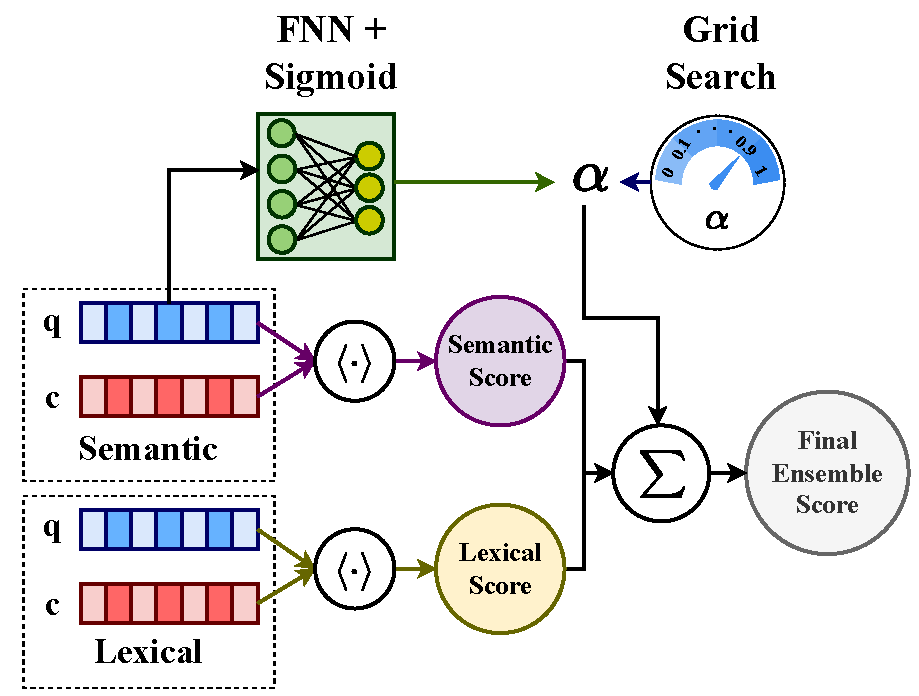
\includegraphics[width=0.45\textwidth]{./images/EnsembleGNN.pdf}
    \vspace{-2mm}
    \caption{Ensemble of lexical and semantic models. $\alpha$ can be tuned either via grid-search or dynamically learned via FFN.}
    \label{fig:ensemble}
    \vspace{-5mm}
\end{figure}


%\subsection{Paragraph-level retrieval methods}
%\vspace{2mm}
\vspace{1mm}
\noindent\underline{\textbf{Paragraph-level methods:}} %Since both the query and candidate documents are large, they can be split into natural paragraphs. 
%Since, original query and candidate documents are organized in the form of paragraphs. 
% We apply unsupervised methods directly at paragraph level for a query-candidate pair, and then aggregate the paragraph-level scores into a single document level score. Specifically, for a query $q$ having $n_q$ paragraphs and a candidate $c$ having $m_c$ paragraphs, we obtain a paragraph level $n_q \times m_c$ score matrix $M$. Then, we use two different aggregation measures:
% (i)~\textit{Max-All:} $\textrm{max}(M)$, and
% (ii)~\textit{Max-Sum:} $\sum_{i=1}^{n} \textrm{max}(M_i)$.
% We obtain the paragraph-level scores through BM25 2-gram and SAILER. We did not experiment with higher order n-grams since it was computationally prohibitive.
% Also, we could not fine-tune at the paragraph-level setup since we do not have the gold-standard information at the paragraph level.
We apply unsupervised methods at the paragraph level for each query–candidate pair, and then aggregate scores into a document-level score. For a query $q$ with $n_q$ paragraphs and candidate $c$ with $m_c$ paragraphs, we compute an $n_q \times m_c$ score matrix $M$. We use two aggregation measures: (i)~\textit{Max-All:} $\max(M)$, and (ii)~\textit{Max-Sum:} $\sum_{i=1}^{n_q} \max(M_i)$. We obtain Paragraph-level scores via BM25 2-gram and SAILER; higher-order n-grams were not attempted due to computational cost. Fine-tuning was also infeasible, as we do not have the ground-truth information at the paragraph level.


\begin{figure*}[t]
    \centering
    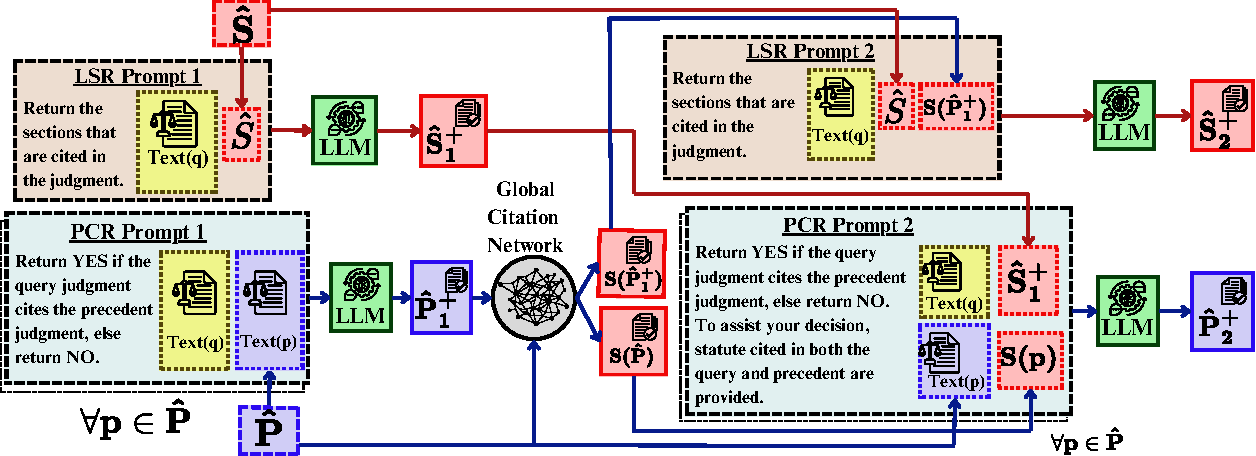
\includegraphics[scale=0.7]{./images/LLM_Reranking.pdf}
    %\includegraphics[width=\linewidth,height=5cm]{./images/EnsembleGNN.png}
    \vspace{-2mm}
    \caption{Proposed two-stage LLM prompting approach}
    \label{fig:llm-two-stages}
    \vspace{-3mm}
\end{figure*}

% \begin{figure}
%     \centering
%     \includegraphics[scale=0.15]{./images/demo_image.png}
%     %\includegraphics[width=\linewidth,height=5cm]{./images/EnsembleGNN.png}
%     \caption{Pipeline of the Ensemble-based approaches. QS and CS represent query and candidate semantic embeddings, while QL and CL represent the query and candidate lexical embeddings.}
%     \label{fig:ensemble}
%     \vspace{-5mm}
% \end{figure}
% \subsection{Ensemble of Lexical \& Semantic Methods} \label{sec:method/ensemble}
%\vspace{2mm}

\vspace{1mm}
\noindent\underline{\textbf{Ensemble of Lexical and Semantic Methods:}}
Combining lexical and semantic features can improve retrieval tasks~\citep{bruch2023fusionhybrid,sumathy2016hybridknowledge,mandikal2024sparsedensehybrid}. In the simplest form, we combine prediction scores for a query–candidate pair $(q,c)$ from lexical and semantic methods, where $c \in \mathcal S$ for LSR, or $c \in \mathcal P$ for PCR (see Fig.~\ref{fig:ensemble}). Formally, 
\vspace{-2mm}
\begin{align*}
\mathcal E(q,c) &= \alpha \times \textrm{Z-Norm}(\Sigma(q,c)) \\
   &\quad + (1 - \alpha) \times \textrm{Z-Norm}(\Lambda(q,c))
\end{align*}

\vspace{-2mm}
\noindent where $\mathcal E$ is the ensemble, $\Sigma$ the semantic method, $\Lambda$ the lexical method, and $\alpha$ a hyperparameter. As model scores vary in range, we apply Z-score normalization across all candidates per query. We use BM25 5-gram as the lexical method, and Event-GNN or Para-GNN as the semantic method.
We use the following two \textit{strategies to decide the optimal value of $\alpha$}:


\noindent\textbf{(1) Grid Search:} We vary the values of $\alpha = \{0, 0.1, \ldots, 0.9, 1\}$ for each task to determine the optimal value over the validation set. %This is done independently for statutes and precedents, and the optimal $\alpha$ value is used over the test set.

\noindent\textbf{(2) Dynamic $\mathbf{\alpha}$:} 
% In this approach, we try to learn the optimal $\alpha$ for each query by employing a feed-forward network (FFN) with sigmoid activation over the query embedding obtained from the semantic method. In the joint tuning setup, we used two separate FFNs for statute and precedent respectively. Apart from tuning independently and in multi-task learning setup, we tried a sequential approach as well, based on transfer learning. For instance, we took the statute model that was tuned independently, and used that to initialize the model for precedent tuning, and vice versa. This gave us models (obtained separately) for each task that were first trained on the other task to exploit the prospect of transfer learning properties between the two tasks.  We conduct in-depth analysis regarding the optimal $\alpha$ value for the different ensemble methods (see App.~\ref{app:gridsearch}).
In this approach, we learn the optimal $\alpha$ per query using a feed-forward network (FFN) with sigmoid activation over the query embedding from the semantic method. In joint tuning, separate FFNs are used for LSR and PCR. Beyond independent and multi-task setups, we also tested a sequential transfer-learning strategy: e.g., initializing the precedent model with the independently tuned statute model, and vice versa. This yielded task-specific models pre-trained on the other task, leveraging cross-task transfer. For further analyses of optimal $\alpha$ values, see App.~\ref{app:optimal-alpha}.

\vspace{1mm}
\noindent\underline{\textbf{Using LLMs for re-ranking:}} 
% Recently, LLMs have shown promising results for retrieval tasks.
% However, since the number of candidates in our setting is large and the texts of queries (and precedents in case of PCR) are very long, it makes it challenging to use LLM as a first-stage retriever. However, LLMs can be used as second-stage re-rankers, by re-ranking a limited number of candidates (say top $k$ candidates as given by any first stage retrieval model). Given the top-$k$ ranked list of candidates ($\hat{C}_k(q) = [c_{q_1}, c_{q_2}, \ldots, c_{q_k}]$) for a given query $q$ by a first stage retriever model $\mathcal M$, we ask the LLM $\mathcal G$ to give a binary relevance score $\mathcal G(q, c_{q_i}) \in \{0,1\}$ for each candidate in the top-$k$. All the subsequent notations are defined from the perspective of a single query $q$ and single chosen $k$ value, thus, for brevity, let us represent $\hat{C}_k(q)$ as $\hat C$.
% We then partition the top-$k$ ranked list as $\hat{C}^+ = \{c_{q_i} \mid \mathcal G(q, c_{q_i}) = 1\}$, and $\hat{C}^- = \{c_{q_i} \mid \mathcal G(q, c_{q_i}) = 0\}$. It is ensured that the original ordering (as per $\hat{C}$) is maintained between the candidates in both $\hat{C}^+$ and $\hat{C}^-$. Thereon, the re-ranked list becomes $\tilde{C}_k(q)$ or $\tilde{C} = \{\hat{C}^+, \hat{C}^-\}$. This ensures that the relevent candidates predicted by the LLM are ranked above those predicted as not relevant. We use a two-stage re-ranking pipeline for both tasks (Fig. ~\ref{fig:llm-two-stages}). % and described in detail below.
Recently, LLMs have shown strong results for retrieval. However, due to the large candidate space and the long texts of queries (and precedents in PCR), they are impractical as first-stage retrievers. Thus, we employ LLMs as second-stage re-rankers. A first-stage retriever $\mathcal M$ returns the top-$k$ list for query $q$:
\vspace{-2mm}
\[\hat{C}_k(q) = [c_{q_1}, c_{q_2}, \ldots, c_{q_k}].\]

\vspace{-2mm}
\noindent The LLM $\mathcal G$ assigns a binary relevance score $\mathcal G(q,c_{q_i}) \in \{0,1\}$ for each candidate. For brevity, let $\hat C := \hat{C}_k(q)$. We then partition $\hat C$ as
\vspace{-2mm}
\begin{align*}
\hat C^+ &= \{c_{q_i} \mid \mathcal G(q,c_{q_i})=1\}, \\
\hat C^- &= \{c_{q_i} \mid \mathcal G(q,c_{q_i})=0\},
\end{align*}

\vspace{-2mm}
\noindent while preserving the original ordering from $\hat C$ within both subsets. By construction,  $|\hat C^+| + |\hat C^-| = k$.
The final re-ranked list is
\vspace{-2mm}
\[\tilde C_k(q) = [\hat C^+, \hat C^-].\]

\vspace{-2mm}
\noindent This ensures that all LLM-predicted relevant candidates precede the non-relevant ones.  We adopt a two-stage re-ranking approach for both tasks. Fig.~\ref{fig:llm-two-stages} shows the entire pipeline for this.

\vspace{1mm}
\noindent\textbf{First-stage prompting:} 
% We first perform an initial stage of re-ranking, where LSR and PCR are performed independently. For statutes, for a given query $q$, we pass the full query text along with the names of \textit{all} the top-$k$ statutes $\hat S$ in the same prompt, and ask the LLM to directly return the set of statutes it considers relevant $\hat{S}_1^+ = \textrm{LLM}(\textrm{Text}(q), \hat{S})$. This approach is conditioned on the fact the LLM already has a prior knowledge of all the statutes $s \in \mathcal S$, and thus it already knows the statute texts. 
% For precedents, the LLM may not know the text of the precedent, and thus we pass the query and precedent text for each precedent $p$ in the top-$k$ precedents $\hat{P}$ in pair-wise fashion and ask it to predict if the pair is relevant. Thus, $\mathcal G_1(q, p) = \textrm{LLM}(\textrm{Text}(q), \textrm{Text}(p))$ and $\hat P_1^+ = \{p \mid p \in \hat P, \mathcal G_1(q,p)=1\}$.
We first perform an initial re-ranking stage where LSR and PCR are handled independently. For statutes, given a query $q$, we pass the full query text along with the names of all top-$k$ statutes $\hat S$ in a single prompt and ask the LLM to return the relevant subset: \vspace{-2mm} 
\[
\hat S_1^+ = \textrm{LLM}(\textrm{Text}(q), \hat S).
\]

\vspace{-2mm}
\noindent This assumes the LLM has prior knowledge of all statutes $s \in \mathcal S$, and therefore already knows their texts. 
For precedents, since the LLM may not know the precedent texts, we pass the query and each candidate precedent $p \in \hat P$ (top-$k$ precedents) in a pairwise fashion, asking if the pair is relevant:
\vspace{-2mm}
\begin{align*}
\mathcal G_1(q,p) &= \textrm{LLM}(\textrm{Text}(q), \textrm{Text}(p)), \\
\hat P_1^+ &= \{p \mid p \in \hat P, \ \mathcal G_1(q,p)=1\}.
\end{align*}

\vspace{-1mm}
\noindent\textbf{Second-stage prompting:} 
% From the first stage prompting, we obtained the initial predictions $\hat S_1^+$ and $\hat P_1^+$ for LSR and PCR respectively.
% In the second stage, we wish to utilize the relationship between LSR and PCR in a sequential fashion, using the outputs of one task to try improve the other. For performing LSR, we first take the positive precedents of PCR re-ranking (first stage), $\hat{P}_1^+$, and collect all ground-truth statutes cited by these precedents $S(\hat{P}_1^+) = \cup_{p \in \hat{P}_1^+} S(p)$, where the $S(.)$ function represents the mapping from any query, or precedent, to its ground-truth statutes. This ground-truth information is known to us during test time since precedents are not masked. These additional statutes are passed to the prompt along with the top-$k$ statute ranked list $\hat S$, to obtain the second-stage re-ranked predictions: $\hat{S}_2^+ = \textrm{LLM}(\textrm{Text}(q), \hat{S} \cup S(\hat{P}_1^+))$. We effectively increase the re-ranking range of the LLM in an informed way, utilizing the connection between precedents and the ground-truth cited statutes. % cited by them.
From the first-stage prompting, we obtain the initial predictions $\hat S_1^+$ and $\hat P_1^+$ for LSR and PCR respectively.  
In the second stage, we leverage the relationship between LSR and PCR sequentially, using the output of one task to improve the other. For LSR, we take the positive precedents from first-stage PCR re-ranking ($\hat P_1^+$) and collect all ground-truth statutes cited by these precedents:
\vspace{-2mm}
\[
S(\hat P_1^+) = \bigcup_{p \in \hat P_1^+} S(p),
\]

\vspace{-2mm}
\noindent where $S(\cdot)$ denotes the mapping from any query or precedent to its ground-truth statutes. This ground-truth is available at test time since precedents are not masked.  
These additional statutes are then passed to the prompt, together with the top-$k$ statute list $\hat S$, to obtain the second-stage predictions:
\vspace{-2mm}
\[
\hat S_2^+ = \textrm{LLM}(\textrm{Text}(q), \hat S \cup S(\hat P_1^+)).
\]

\vspace{-1mm}
\noindent Thus, we expand the re-ranking range of the LLM in an informed manner, exploiting the connection between precedents and their cited statutes.


% \noindent For second-stage precedent re-ranking, we first consider the positive statutes $\hat{S}_1^+$ for the query $q$ as per LCR first-stage re-ranking, and the ground truth statutes $S(p)$ for a precedent $p$, and pass these names to the prompt along with the texts of $q$ and $p$ to get the second-stage PCR mapping $\mathcal G_2(q,p) = \textrm{LLM}(\textrm{Text}(q), \hat{S}_1^+, \textrm{Text}(p), S(p)), \forall p \in \hat{P}$, and thus $\hat P_2^+ = \{p \mid p \in \hat P, \mathcal G_2(q,p)=1\}$. The idea here is that the LLM should be able to exploit the statute information to better judge relevance between $q$ and $p$ for PCR. %We use the predicted statutes for the query and the gold-standard statutes for the precedent.
\noindent For second-stage precedent re-ranking, we use the positive statutes $\hat S_1^+$ for query $q$ (from first-stage LSR) together with the ground-truth statutes $S(p)$ for each precedent $p$. These statute names are passed to the prompt along with the texts of $q$ and $p$, yielding the second-stage PCR mapping:
\vspace{-2mm}
\begin{align*}
\mathcal G_2(q,p) &= \textrm{LLM}\big(\textrm{Text}(q), \hat S_1^+, \nonumber \\
&\quad\ \ \textrm{Text}(p), S(p)\big), \quad \forall p \in \hat P, \\
\hat P_2^+ &= \{p \mid p \in \hat P, \mathcal G_2(q,p)=1\}.
\end{align*}

\vspace{-2mm}
\noindent The intuition is that by conditioning on statute information, the LLM can better assess the relevance of precedents to the query in PCR.
All prompts are shown in brief in Fig.~\ref{fig:llm-two-stages} (full prompts in App.~\ref{app:prompts}).

% \vspace{2mm}
% \noindent\underline{\textbf{Setup and Hyperparameters:}}
% For BM25-based experiments, we used different n-grams ($n=2,3,4,5$). In case of the fine-tuning approaches, we use a contrastive learning setup, with BM25 hard negatives and in-batch negative sampling. We used  AdamW~\citep{loshchilov2017adamw} optimizer and a linear scheduler. \paul{For re-ranking, we used GPT-4.1 and chose top $k=20$ for statutes and $k=10$ for precedents.} For more details see App. \ref{app:implementation}. %Exact details of the setup and hyper-parameter settings are provided in Appendix~\ref{app:implementation}.
% \vspace{2mm}
% \noindent\textbf{Grid Search:} We vary the values of $\alpha = \{0, 0.1, \ldots, 0.9, 1\}$ to determine the optimal value over the validation set. This is done independently for statutes and precedents, and the optimal $\alpha$ value is used over the test set.

% \vspace{2mm}
% \paul{\noindent\textbf{Dynamic $\mathbf{\alpha}$:} In this approach, we try to learn the optimal $\alpha$ for each query by employing a feed-forward network (FFN) with sigmoid activation over the query embedding obtained from the semantic method. In the joint tuning setup, we used two separate FFNs for statute and precedent respectively. Apart from tuning independently and in multi-task learning setup, we tried a pipeline approach as well. We took the statute model tuned independently, and used that to initialize the model for precedent tuning, and vice versa for statute tuning. This gave us models (obtained separately) for each task that were first trained on the other task to exploit the prospect of transfer-learning properties between the two tasks.} 

%\subsection{Usage of LLMs in retrieval methods}
% \vspace{2mm}
% \noindent\underline{\textbf{Usage of LLMs in retrieval methods:}} %Generative LLMs have transformed the NLP space lately, producing superior performance on many tasks. However, 
% It is difficult to use LLMs directly for retrieval purposes, since the model must be fed the query text as well as \textit{all the candidate texts} in the same prompt window. 
% This is not straight-forward in the legal domain since we have a large number of candidates, and the texts are quite lengthy. We instead use LLMs to restructure the input for downstream retrieval models, by creating events  or summaries. 
%We instead use LLMs to restructure the input for downstream retrieval models, by creating events (in Event-GNN)
%(Section~\ref{sec:method/semantic}) 
%or summaries, as described above. %(Section~\ref{sec:method/summary}).

% \noindent\underline{\textbf{Using LLMs for re-ranking:}} 
% \paul{It is difficult to use LLMs as first stage retrievers, since the number of candidates is large and the texts of queries (and precedents in case of PCR) are very long. However, LLMs can be used as second-stage re-rankers, by re-ranking a limited number of candidates (say top $k$ candidates as given by any first stage retrieval model) for each query. Given the top-$k$ ranked list of candidates for a given query $q$ by a first stage retriever model $\mathcal M$, $\hat{C}_k(q) = [c_{q_1}, c_{q_2}, \ldots, c_{q_k}]$, we ask the LLM $\mathcal G$ to give a binary relevance score $\mathcal G(q, c_{q_i}) \in \{0,1\}$ for each candidate in the top-$k$.}
% \paul{\textit{All further notations are defined from the perspective of a single query $q$ and single chosen $k$ value, thus, for brevity, let us represent $\hat{C}_k(q)$} as $\hat C$.}
% \paul{We then partition the top-$k$ ranked list as $\hat{C}^+ = \{c_{q_i} \mid \mathcal G(q, c_{q_i}) = 1\}$, and $\hat{C}^- = \{c_{q_i} \mid \mathcal G(q, c_{q_i}) = 0\}$. It is ensured that the original ordering (as per $\hat{C}$) is maintained between the candidates in both $\hat{C}^+$ and $\hat{C}^-$. Thereon, the re-ranked list becomes $\tilde{C}_k(q)$ or $\tilde{C} = \{\hat{C}^+, \hat{C}^-\}$. This ensures that the candidates predicted relevant by the LLM are ranked ahead of those predicted as not relevant.
% We use a two-stage re-ranking pipeline for both tasks, which is shown in Figure~\ref{fig:llm-two-stages}, and described in detail below.}

% \noindent\textbf{First-stage prompting:} \paul{We first perform an initial stage of re-ranking, where LSR and PCR are performed independently. For statutes, for a given query $q$, we pass the full query text along with the names of \textit{all} the top-$k$ statutes $\hat S$ in the same prompt, and ask the LLM to directly return the set of statutes it considers relevant $\hat{S}_1^+ = \textrm{LLM}(\textrm{Text}(q), \hat{S})$. This approach is conditioned on the fact the LLM already has a prior knowledge of all the statutes $s \in \mathcal S$, and thus it already knows the statute texts. 
% For precedents, the LLM may not know the text of the precedent, and thus we pass the query and precedent text for each precedent $p$ in the top-$k$ precedents $\hat{P}$ in pair-wise fashion and ask it to predict if the pair is relevant. Thus, $\mathcal G_1(q, p) = \textrm{LLM}(\textrm{Text}(q), \textrm{Text}(p))$ and $\hat P_1^+ = \{p \mid p \in \hat P, \mathcal G_1(q,p)=1\}$.}


% \noindent\textbf{Second-stage prompting:} 
% \paul{From the first stage prompting, we have obtained the initial predictions $\hat S_1^+$ and $\hat P_1^+$ for LSR and PCR respectively.}
% \paul{In the second stage, we wish to utilize the relationship between LSR and PCR in a pipeline fashion, using the outputs of one task to try improve the other. For performing LSR, we first take the positive precedents of PCR re-ranking (first stage), $\hat{P}_1^+$, and collect all ground-truth statutes cited by these precedents $S(\hat{P}_1^+) = \cup_{p \in \hat{P}_1^+} S(p)$, where the $S(.)$ function represents the mapping from any query, or precedent, to its ground-truth statutes. This ground-truth information is known to us during test time since precedents are not masked. Thereon, we simply pass these additional statutes to the prompt along with the top-$k$ statute ranked list $\hat S$, to obtain the second-stage re-ranked predictions: $\hat{S}_2^+ = \textrm{LLM}(\textrm{Text}(q), \hat{S} \cup S(\hat{P}_1^+))$. We effectively increase the re-ranking range of the LLM in an informed way, utilizing the connection between precedents and the ground-truth statutes cited by them.}

% \paul{For second-stage precedent re-ranking, we first consider the positive statutes $\hat{S}_1^+$ for the query $q$ as per LCR first-stage re-ranking, and the ground truth statutes $S(p)$ for a precedent $p$, and pass these names to the prompt along with the texts of $q$ and $p$ to get the second-stage PCR mapping $\mathcal G_2(q,p) = \textrm{LLM}(\textrm{Text}(q), \hat{S}_1^+, \textrm{Text}(p), S(p)), \forall p \in \hat{P}$, and thus $\hat P_2^+ = \{p \mid p \in \hat P, \mathcal G_2(q,p)=1\}$. The idea here is that the LLM should be able to exploit the statute information to better judge relevance between $q$ and $p$ for PCR. We use the predicted statutes for the query and the gold-standard statutes for the precedent.}

% \vspace{2mm}
% \noindent\underline{\textbf{Setup and Hyperparameters:}}
% For BM25-based experiments, we used different n-grams ($n=2,3,4,5$). In case of the fine-tuning approaches, we use a contrastive learning setup, with BM25 hard negatives and in-batch negative sampling. We used  AdamW~\citep{loshchilov2017adamw} optimizer and a linear scheduler. \paul{For re-ranking, we used GPT-4.1 and chose top $k=20$ for statutes and $k=10$ for precedents.} For more details see App. \ref{app:implementation}. %Exact details of the setup and hyper-parameter settings are provided in Appendix~\ref{app:implementation}.



% \begin{table*}
%     \centering
%     \small
%     \begin{tabular}{p{0.18\textwidth}p{0.30\textwidth}cccccc}
%          \hline
%          \textbf{Ensemble Method} & \textbf{Setting} & \multicolumn{3}{c}{\textbf{Statutes}} & \multicolumn{3}{c}{\textbf{Precedents}} \\ 
%           & & \textbf{F1} & \textbf{MAP} & \textbf{MRR} & \textbf{F1} & \textbf{MAP} & \textbf{MRR} \\ \hline

%           Event-GNN + BM25 & Grid Search & \textbf{33.87} & \textbf{45.17} & \textbf{67.26} & 34.45 & 43.32 & 58.76 \\
%           & Dynamic $\alpha$, finetune separately & 30.29 & 40.97 & 61.51 & 35.60 & 45.86 & 60.89 \\
%           & Dynamic $\alpha$, finetune multi-task & 25.62 & 31.97 & 57.01 & 35.63 & 45.18 & 60.51 \\ \hline
%           Para-GNN + BM25 & 5-gram, Grid Search & 28.10 & 36.14 & 59.57 & \textbf{36.93} & \textbf{48.62} & \textbf{62.83} \\
%           & Dynamic $\alpha$, finetune separately & 27.05 & 35.20 & 59.67 & 36.91 & 48.53 & 62.61 \\
%           & Dynamic $\alpha$, finetune multi-task & 27.01 & 33.57 & 59.00 & 36.57 & 48.18 & 62.14 \\ \hline
%           Para-GNN (summaries) + BM25 & Grid Search & 36.17 & 48.64 & 70.49 & 36.35 & 48.27 & 61.76 \\ \hline
%     \end{tabular}
%     \caption{Results of ensemble methods for both LSR and PCR tasks. Best value for each metric in boldface. \paul{Ensemble summaries fine-tuning TBD}}
%     \label{tab:ensemble}
%     \vspace{-5mm}
% \end{table*}



% \begin{table*}
%     \centering
%     \small
%     \begin{tabular}{lcccccc}
%         \hline
%         \textbf{Method} & \multicolumn{3}{c}{\textbf{Statutes}} & \multicolumn{3}{c}{\textbf{Precedents}} \\
%         & Lexical & Semantic & Ensemble & Lexical & Semantic & Ensemble \\ \hline
%         Para-GNN (GridSearch) & 16.98 & 20.72 & 28.10 & 33.29 & 24.54 & 36.93 \\
%         Para-GNN (dynamic) &  16.98 & 20.72 & 27.05 & 33.29 & 24.54 & 36.91 \\ \hline
%         Event-GNN (GridSearch) & 16.98 & 28.67 & 33.87 & 33.29 & 12.08 & 34.45 \\ 
%         Event-GNN (dynamic) &   &  &  &  &  & \\ \hline
%     \end{tabular}
%     \caption{Performance (macro-F1@K in \%) of ensemble models compared with the default lexical and semantic approaches \sg{I find the format of this table very confusing. It seems the entire row is for the method stated on the left, but it is not so. Why can we not use the same format as in Table~\ref{tab:results}?}}
%     \label{tab:ensemble}
% \end{table*}






% \subsection{Ensemble of Lexical and Semantic Methods}

% We also experimented with an ensemble setup to combine the effect of lexical and semantic methods. In the simplest setup, we can combine the prediction (score) of assigned to a particular (query, candidate) pair by a lexical method with that given by semantic methods. Formally, $\textrm{Score}(Q,C) = \alpha \times \textrm{Semantic Norm Score}(Q,C) + (1 - \alpha) \times \textrm{Lexical Norm Score}(Q,C)$. We need the normalized scores since the default scores coming from the models can be of different scales; here we performed Z-score normalization across all candidates for each query. In the ensemble approaches, we used BM25 5-gram as the lexical method and Event-GNN or RR-GNN as the semantic method.

% \noindent\textbf{Grid Search for Best $\alpha$:} We vary the values of $\alpha = \{0, 0.1, 0.2, \ldots, 0.9, 1\}$, and determine the optimal setting.

% \noindent\textbf{Dynamic $\alpha$:} We tune a feed-forward network with sigmoid activation on top of the semantic embeddings to generate the $\alpha$ value dynamically according to each query. The semantic methods are fine-tuned along with the linear layer.



